\chapter{Implementation}
\label{ch:implementation}


In this chapter, details of the implementation practical part of the study is discussed. The architecture, modules, development tools, installation, and configurations of such part are the main role of this chapter.    
\section {Architecture}
The design of the architecture was planned based on the Input-Process-Output Model. It can be also considered as a black-box solution where the solution processes the input, then it delivers the output once it is ready. follows is the discussion of those 3 phases, described in Figure \ref{Fig:Architecture} : 
 \begin{figure}[ht]
	\begin{center}
		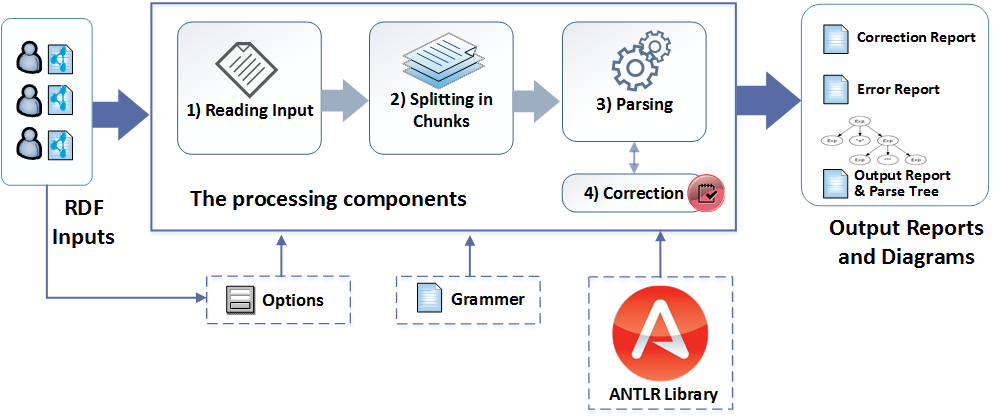
\includegraphics[scale=0.5,angle=0]{images/Architecture}
		\caption{The proposed solution architecture}
		\label{Fig:Architecture}
	\end{center}
\end{figure}
 \begin{itemize}
 \item \textbf {Input}: It is the role of the user to supply an RDF text with certain options, such as 1) enabling/disabling of the error correction, 2) showing an error report of JSON \footnote{\href{https://www.json.org/}{JSON}} or text format, and 3) concealing/showing up the parse tree.
\item \textbf{Process}: starts with preparing the input ready to be parsing in the following flow: 1)it reads the input, 2) slices it into smaller pieces if needed, 3) parses the input itself or each slice, and 4) corrects some detected syntax errors. This phase was built based on a predefined grammar, it requires ANTLR library for parsing, and some options from the user to activate/deactive some features of the solution.   
\item \textbf{Output}: provides the reports after processing the input, including 1) an errors report to announce the detected syntax errors, 2) a correction report to report the recovered syntax errors, and 3) an output file after healing some of the detected syntax errors, and 4) a frame contains the parse tree. Both of the correction report and the output file need the enabling of the error correction feature to be generated. 
\end{itemize}



\section {Modules} 

	\begin{figure}[ht]
	\begin{center}
		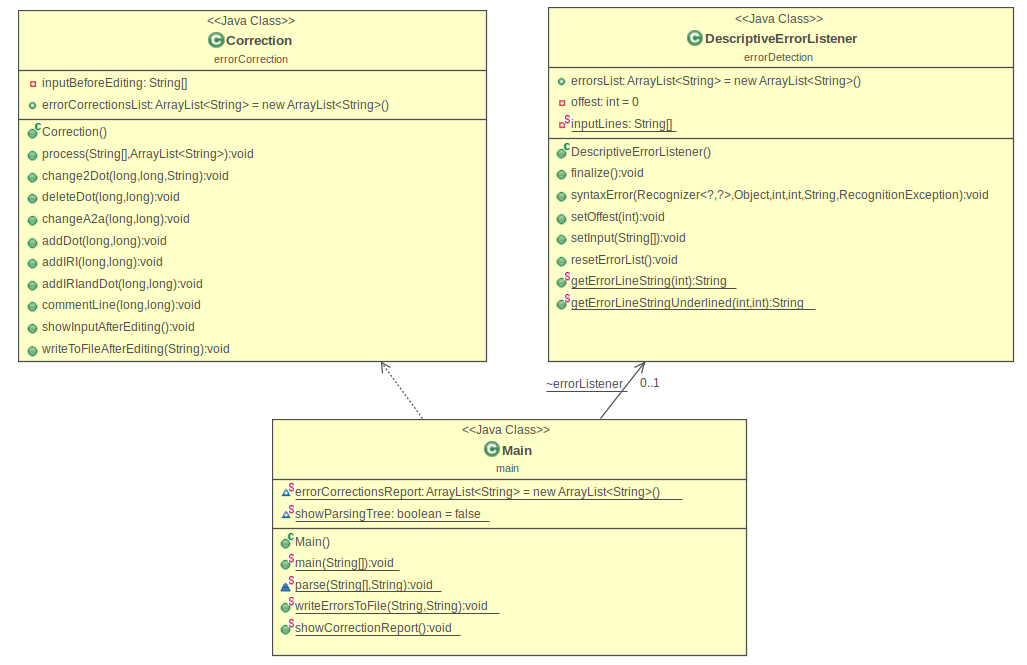
\includegraphics[scale=0.5,angle=0]{images/modules.png}
		\caption{UML diagram for the major modules in the proposed solution}
		\label{Fig:UML}
	\end{center}
\end{figure}

After briefing the proposed solution architecture, It is the time to cover it in more details by shedding light onto those modules which represent the pillars of such solution. {Figure \ref{Fig:UML}} establishes a UML diagram for the most significant modules in this solution, represented into 3 modules: Main, Error Detection, and Error Correction. The following text discusses those modules plus Core module. It is worth to be noted that Core module is not shown in {figure \ref{Fig:UML}} to facilitate the understanding of the main modules, otherwise it would be complex, furthermore, Core is automatically generated module by ANTLR based on the given grammar, thereby few changes were coded in the module:  
 \begin{enumerate}[]
 \item \textbf {Core}: is automatically generated by ANTLR based on the grammar defined appendix \ref{ch:appendix}. It encloses the parsing classes such as Parser, Lexer, Error Collector, Parse Tree Creator.   
\item \textbf{Errors Detection}: listens to the generated error messages by the parser. conventionally, while parsing if the parser detects syntax errors it sends a detail of the error to an error collector if one was defined.   
\item \textbf {Error Correction}: corrects those syntax errors which have only a well-know solution, this module was codded. The error message plays an important role to identify whether it can such error can be corrected or not. A global list stores all detected syntax errors messages and their location in the input (line number and column number) and this modules has predefined messages. if any of the detected error message matches any of the predefined messages, then such error can be healed and recovered.
\item \textbf{Main}: is the executive part which combines input, output, and processing components. It receives the input text, and if it is large (for example, more than 1 million lines), it is segmented into one or more chunks based on its size. Each chunk is handled separately in regards of parsing, error detection, as well as in error correction.

\end{enumerate} 

%TODO:check here how to adjust the vertical space 
\vspace{-5mm}

\section{Real-World Use Cases}
In this section, some of use cases tackled in this study to detect syntax errors in RDF input and  the method of error correction of some of those detected syntax error will be exposed. As a start, let's begin with a Turtle example which has no syntax errors, then some syntax errors can be included, then the process of handling them can explained. 
	\vspace{5mm} %5mm vertical space

Listing \ref{lst:turtleExample} shows a Turtle example without syntax errors. First 4 lines are directives or prefixes declaration. 
\
\begin{lstlisting}[label=lst:turtleExample, numbers=left, caption={RDF example in Turtle serialization format}]
<@\textcolor{blue}{@prefix}@>  <@\textcolor{red}{rdf}@>: <@\textcolor{orange}{<http://www.w3.org/1999/02/22-rdf-syntax-ns#>}@> .
<@\textcolor{blue}{@prefix}@>  <@\textcolor{red}{rdfs}@>:  <@\textcolor{orange}{<http://www.w3.org/2000/01/rdf-schema#>}@> .
<@\textcolor{blue}{@prefix}@>  <@\textcolor{red}{ex}@>:  <@\textcolor{orange}{<http://example.org/>}@> .
<@\textcolor{blue}{@prefix}@>  <@\textcolor{red}{zoo}@>:   <@\textcolor{orange}{<http://example.org/zoo/> }@> .
<@\textcolor{red}{ex}@>:dog1  <@\textcolor{red}{rdf}@>:type  <@\textcolor{red}{ex}@>:animal .
<@\textcolor{red}{ex}@>:cat1  <@\textcolor{red}{rdf}@>:type  <@\textcolor{red}{ex}@>:cat ;
         <@\textcolor{red}{rdfs}@>:label   <@\textcolor{green}{"Lusi"@en}@> .
<@\textcolor{red}{ex}@>:cat  <@\textcolor{red}{rdfs}@>:subClassOf  <@\textcolor{red}{ex}@>:animal .
<@\textcolor{red}{zoo}@>:host  <@\textcolor{red}{rdfs}@>:range  <@\textcolor{red}{ex}@>:animal .
<@\textcolor{red}{ex}@>:zoo1  <@\textcolor{red}{zoo}@>:host  <@\textcolor{red}{ex}@>:cat2 .
\end{lstlisting}










